\documentclass[../main.tex]{subfiles}
\graphicspath{{\subfix{../Figures/}}}

\begin{document}

\chapter{Methods}
\label{ch:methods}

\section{Problem 1: Multi-class extension}

\subsection{Problem statement}

The authors of \ls{} solve the following problem \cite{cohenGifsplanation2022}:

Let $f: \R^\inputdim \to [0, 1]$ be a binary classifier such that $f(x)$ outputs the predicted probability of $x$ being in class 1.
Let $x$ be a point that is predicted to be of class 0, \ie{} such that $f(x) < \frac{1}{2}$.
Find a path starting at (or around) $x$ and ending at a point $\CF{x}$ for which $f(\CF{x}) > \frac{1}{2}$ such that the path is sufficiently simple and easily comprehensible by a human.

They propose building a latent representation $\autoencoder = (\enc, \dec)$, letting $z = \enc(x)$ and computing the gradient of the classifier in that latent space:
$\nabla_z f(\dec(z))$.
Then they can recover a potential counterfactual by shifting the latent along the gradient: $\CF{x} = \dec(z + \lambda \nabla_z f(\dec(z)))$ where $\lambda$ is some positive real number.
Since the gradient gives the direction of steepest ascent, going in this direction is the best strategy to increase $f(\dec(z))$ and therefore obtain a valid $\CF{x}$.

In the case of a binary classifier that outputs a scalar, this might be sufficient. However, in multi-class problems where $f$ outputs a vector in $\R^\outputdim$ there are several possible choices of functions of which we could compute the gradient.
To see this, we reformulate the latent shift strategy with a generic loss that accounts for validity, denoted by $\lossval$:

Let $f$ be the classifier of interest, which outputs logits in $\R^\outputdim$ rather than a probability mass.
Given $x \in \inputspace$ and an autoencoder $\autoencoder = (\enc, \dec)$, a counterfactual path can be generated by computing the gradient of the validity loss $\lossval$ and perturbing $z = \enc(x)$ along the opposite of the gradient (that is, in the direction of steepest \emph{descent}) so as to minimize $\lossval$:
$\CF{x} = \dec(z - \lambda \nabla_z \lossval(z))$.

In vanilla \ls{}, the validity loss would then be $\lossval(z) = - \sigma(f(\dec(z)))$ where $\sigma$ denotes the sigmoid function, or any other increasing differentiable function that outputs a number in $[0, 1]$.

Hence, our problem is as follows:
Find a validity loss $\lossval$ that, for a given $x \in \inputspace$, gives rise to a class-changing path in input space when used in a gradient-based path generation method such as the one described above.

\subsection{Proposed solutions}

Note that this extension to the multi-class setting means that we have a choice to specify a given target class: we might also prefer to simply change the class, without preference of target class. In our analysis we focus on the case where a target class is specified.

In order to mimic the solution discussed in \cite{cohenGifsplanation2022}, we could use
\begin{equation}
    \lossval(z) = -\softmax(f(\dec(z)))_\target,
\end{equation}
\ie{} the component of the output probability mass corresponding to class $\target$.
As before, the codomain is $[0, 1]$, and the loss corresponds directly to what we wish to achieve.


% However, because the codomain is small, the gradients computed from this loss could potentially be very small in magnitude and thus unreliable.
% By contrast, a typical loss function used in classification tasks (such as the cross-entropy) often includes a logarithm so that the loss can change more rapidly which promotes larger gradients. \citenote{}
% Hence, we use the cross-entropy instead: $$\lossval = \ce(f(\dec(z)), y_\target).$$
% We call this validity loss \method{TargetLoss}.

% There are other possible variants. For example, one might wish to specify that, if not able to reach the target class, the path should at least get away from the source class. This can be included as follows:
% $$\lossval = \ce(f(\dec(z)), y_\target) - \ce(f(\dec(z)), y_\source).$$
% We call this variant \method{BinaryStretchLoss}.

% Taking this idea further, one might wish that the path should get away from all classes that are not the target, which we could model as follows:
% $$\lossval = \ce(f(\dec(z)), y_\target) - \sum_{c \neq \target} \ce(f(\dec(z)), y_c).$$
% We call this \method{StretchLoss}. 

We could stop there, but in fact other possibilities arise because of the multi-class assumption.

Indeed, in the binary classification case, reaching towards the target class is exactly the same as moving away from the source class, since $p_\source = 1 - p_\target$.
By contrast, in the multi-class setting, different priorities need to be distinguished on a case-by-case basis: is it more important to reach the target (at the risk of potentially staying in the source class) or to get away from the source (at the risk of not reaching the target)?
The natural extension we presented is favoring the first option, but perhaps some variation of it could be preferable.

Thus, we introduce the following alternative loss:
\begin{equation}
    \lossval(z) = -\softmax(f(\dec(z)))_\target
    + \softmax(f(\dec(z)))_\source
\end{equation}
which can be interpreted as adding the constraint of going away from the source as well as going towards the target.

We can validate our intuition, we can compute the gradient of the validity loss:
\begin{align}
    \grad{\lossval}{z}
    =  \grad{}{z} \left( - \softmax(f(\dec(z)))_\target + \softmax(f(\dec(z)))_\source \right)
\end{align}

Because $z$ will only ever appear within $f(\dec(z))$, let $u = f(\dec(z))$; by the chain rule, we have $\grad{\lossval}{z} = \grad{\lossval}{u} \grad{u}{z}$.
$\grad{u}{z}$ does not change with the loss so we focus on $\grad{\lossval}{u}$:
\begin{align}
    \grad{\lossval}{u}
    =  \grad{}{u} \left( - \softmax(u)_\target + \softmax(u)_\source \right)
\end{align}

{
\newcommand{\eu}[1]{\e^{u_{#1}}}
\newcommand{\seu}{\sum_{c \in \setclasses} \eu{c}}

\begin{align*}
    \grad{\softmax(u)_i}{u_j}
     & = \grad{}{u_j} \frac{\eu{i}}{\seu}                                                 \\
     & = \frac{\grad{\eu{i}}{u_j} \seu - \eu{i} \grad{}{u_j} \seu}{\left( \seu \right)^2} \\
     & = \frac{\delta_{ij} \eu{i} \seu - \eu{i} \eu{j}}{\left(\seu \right)^{2}}           \\
     & = \delta_{ij} \frac{\eu{i}}{\seu} - \frac{\eu{i}}{\seu} \frac{\eu{j}}{\seu}        \\
     & = \softmax(u)_i ( \delta_{ij}  -  \softmax(u)_j)
\end{align*}
}


\section{Problem 2: Path regularization}

\subsection{Problem statement}

A typical requirement on a counterfactual $\CF{x}$ for an input $x$ might be for $\norm{\CF{x} - x}$ to be small, where $\norm{\cdot}$ could be the $L_1$ norm for example \note{cite}.
While this makes sense for methods that produce a discrete set of counterfactuals, we focus on methods that produce \emph{continuous explanation paths}, hence we wish to ensure these requirements are satisfied \emph{along the path}.
In the case of distance, we might wish that the endpoint of the path $\CF{x} = \dec(z_T)$ be close to the starting point, but also that \emph{on the whole} the path $(z_t)_{t=1}^T$ stay as close as possible to the starting point.

In the case of gradient-descent optimization paths, this can be addressed by placing these constraints in the loss function during the computation of the next step: this is the case in \revise{}, where the loss function includes the $L_1$ distance \cite{joshiRealistic2019}:
\begin{equation*}
    \loss_{CF}(z_t) = \lossval(z_t) + \lambda_\text{distance} \norm{\dec(z_t) - x}_1.
\end{equation*}
However, for \ls{} this solution is not appropriate because the gradient is only computed once, for $z = \enc(x)$: even though the first step might be in the right direction, overall the whole path could still go in the wrong direction because the information carried by the gradient is less relevant the further away we go from the input.
In other words, this solution would amount to optimizing not over the path, but over the first step of the path.

Hence, our second problem statement is the following: in the case of gradient-descent methods it makes sense to use losses that take a $z_t$ as input, but how can we constrain a whole path $(z_t)_{t=1}^T$?

\subsection{Proposed solution}

Since we can extend many of the point-wise measures to whole paths in a natural way, \eg{} with the mean or the area-under-curve, we propose using this as a loss on the whole path, which could be used to \emph{train the autoencoder} in addition to its usual loss function.
This added component to the loss can take various forms, and in general we call it \emph{path regularization}. The full process is described with pseudocode in \autoref{algo:pathreg}.
Note that in NF-based autoencoders, the decoder is the inverse of the encoder and thus does not need to be trained like it would in a VAE; this is why we show explicitly only the trainable parameters of $\enc$ (denoted by $\phi$).

\begin{algorithm}
\caption{Learning a normalizing flow latent space by SGD with path regularization}
\label{algo:pathreg}
\KwData{Classifier $f, \autoencoder (\enc_\phi, \dec),$ (training) data, CF loss $\cfloss$, path loss $\pathloss$, path loss regularization coefficient $\lambda_\apath$}
\KwOut{$\phi^*$ that minimizes the $\nll$ and the path loss}
\While{not converged}{
$x \gets \mathtt{get\_input}(\text{data})$ \\
$z \gets \enc_\phi(x)$ \\
$\source \gets f(x)$ \\
$\target \gets \mathtt{random\_target}(x)$ \tcp*{such that $\target \neq \source$}
$\apath \gets \mathtt{generate\_path}_{\cfloss}(z, \source, \target)$ \tcp*{$\apath = (\CF{x}_t)_{t=1}^T$}
$\phi \gets \phi - \nabla_\phi {(\nll(\phi) + \lambda_\apath \pathloss(\apath))}$ \\
}
\end{algorithm}

Since the one obvious constraint on paths is that they should be valid, one way to include this in $\pathloss$ could be to add a count of the number of valid paths in the batch.
Note that class information is indirectly given during the training of the autoencoder, so the autoencoder is dependent on the classification task.
\note{todo}
% This is counter to the \note{todo}.

\section{Robustness of path regularization}

\subsection{Problem statement}

\subsection{Proposed solution}

\section{Metrics}


\section{Datasets}
\label{sec:datasets}

In our experiments we use one custom synthetic dataset generated in a parametrizable way, as well as some real datasets.

We always take out the categorical features and we standardize each feature.

\subsection{\CakeOnSea}

Our analyses were complicated by the impossibility of visualizing counterfactuals for tabular data in general.
Thus, in order to start approaching the problem intuitively, we developed a synthetic dataset with no more than two features that have an influence on the response.
The two features, denoted by $x_0$ and $x_1$, range from 0 to 50, except for the so-called ``dead zone'' which is $[25, 35]^2$, in which there are no points at all.
There are three classes, and the class decision rule is as follows:
\begin{align*}
    (x_0, x_1) \in [35, 45]^2 \implies & y = 2 \\
    x_1 < 25                  \implies & y = 0 \\
    (x_0, x_1) \in \text{dead zone} \lor (x_0, x_1) \notin [0, 50]^2  \implies & y\ \text{unknown} \\
    \text{otherwise} \qquad            & y = 1
\end{align*}
Note that we explicitly refrain from assigning a class if $x = (x_0, x_1)$ is in the dead zone, to simulate a situation with completely unrealistic points.
The decision rule can be visualized in \autoref{fig:cake_on_sea}.

To generate the dataset, we randomly sample points in the $[0, 50]^2$ and then take out points from the dead zone. By default, the sampling distribution is a uniform $\mathcal{U}([0, 50]^2)$.

\begin{figure}[h]
    \centering
    

\tikzset{every picture/.style={line width=0.75pt}} %set default line width to 0.75pt        

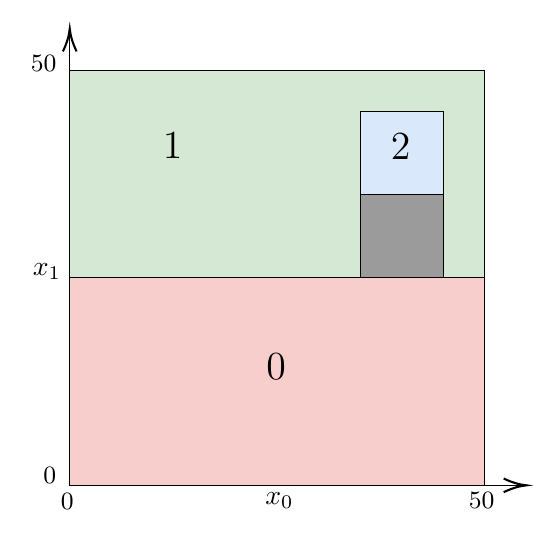
\begin{tikzpicture}[x=0.75pt,y=0.75pt,yscale=-1,xscale=1]
%uncomment if require: \path (0,300); %set diagram left start at 0, and has height of 300

%Shape: Rectangle [id:dp12943827359599314] 
\draw  [fill={rgb, 255:red, 213; green, 232; blue, 212 }  ,fill opacity=1 ] (250,50) -- (450,50) -- (450,150) -- (250,150) -- cycle ;
%Straight Lines [id:da8416607833401318] 
\draw    (250,250) -- (250,32) ;
\draw [shift={(250,30)}, rotate = 90] [color={rgb, 255:red, 0; green, 0; blue, 0 }  ][line width=0.75]    (10.93,-3.29) .. controls (6.95,-1.4) and (3.31,-0.3) .. (0,0) .. controls (3.31,0.3) and (6.95,1.4) .. (10.93,3.29)   ;
%Straight Lines [id:da5577600596159713] 
\draw    (250,250) -- (468,250) ;
\draw [shift={(470,250)}, rotate = 180] [color={rgb, 255:red, 0; green, 0; blue, 0 }  ][line width=0.75]    (10.93,-3.29) .. controls (6.95,-1.4) and (3.31,-0.3) .. (0,0) .. controls (3.31,0.3) and (6.95,1.4) .. (10.93,3.29)   ;
%Straight Lines [id:da17568384394881242] 
\draw    (250,150) -- (450,150) ;
%Shape: Rectangle [id:dp3705541448905584] 
\draw  [fill={rgb, 255:red, 248; green, 206; blue, 204 }  ,fill opacity=1 ] (250,150) -- (450,150) -- (450,250) -- (250,250) -- cycle ;
%Shape: Rectangle [id:dp5334639009219723] 
\draw  [fill={rgb, 255:red, 218; green, 232; blue, 252 }  ,fill opacity=1 ] (390,70) -- (430,70) -- (430,110) -- (390,110) -- cycle ;
%Shape: Rectangle [id:dp05533155300504711] 
\draw  [fill={rgb, 255:red, 155; green, 155; blue, 155 }  ,fill opacity=1 ] (390,110) -- (430,110) -- (430,150) -- (390,150) -- cycle ;

% Text Node
\draw (343.5,185.33) node [anchor=north west][inner sep=0.75pt]  [font=\Large]  {$0$};
% Text Node
\draw (293.6,79) node [anchor=north west][inner sep=0.75pt]  [font=\Large]  {$1$};
% Text Node
\draw (403.5,79.33) node [anchor=north west][inner sep=0.75pt]  [font=\Large]  {$2$};
% Text Node
\draw (343,252) node [anchor=north west][inner sep=0.75pt]    {$x_{0}$};
% Text Node
\draw (231,142) node [anchor=north west][inner sep=0.75pt]    {$x_{1}$};
% Text Node
\draw (244.5,252.67) node [anchor=north west][inner sep=0.75pt]  [font=\small]  {$0$};
% Text Node
\draw (236,240.33) node [anchor=north west][inner sep=0.75pt]  [font=\small]  {$0$};
% Text Node
\draw (230,41.67) node [anchor=north west][inner sep=0.75pt]  [font=\small]  {$50$};
% Text Node
\draw (441,252) node [anchor=north west][inner sep=0.75pt]  [font=\small]  {$50$};


\end{tikzpicture}

\caption{Decision rule for the \CakeOnSea dataset.}
    \label{fig:cake_on_sea}
\end{figure}

\subsection{\ForestCover}

This dataset is taken from the UCI Machine Learning repository \cite{duaUCI2019} and can be found at this URL: \url{https://archive.ics.uci.edu/ml/datasets/Covertype}. 
\note{cite orginal authors}
It contains data on about 580000 trees such as their elevation, their horizontal distance to the nearest surface water features and the type of soil they are in, as well as their species (among seven tree species). There is a total of 13 recorded variables, including the tree species. Of the 12 variables used for prediction, two are categorical, and encoded as one-hot columns.
Because our method does not trivially extend to categorical features yet, we remove the one-hot columns.

\subsection{\WineQuality}

The \WineQuality dataset consists of data on around 6000 wines, such as their pH, their density and their alcohol percentage, as well as a quality rating from 0 to 10.
There are 12 variables including the quality rating column; except for the quality, all of them are numerical.
\note{cite}

In fact, there are no wines with a quality rating of 0, 1, 2 or 10, and 43\% of the rows have a rating of 6 out of 10.
Hence, for our classification task we create the following class mapping:
\begin{itemize}
    \item class 0 corresponds to a quality rating of 5 or lower,
    \item class 1 to a rating of 6,
    \item class 2 to a rating of 7 or higher.
\end{itemize}
With this mapping, around 33\% of data are in class 0, 43\% in class 1 and 18\% in class 2.

\subsection{\OnlineNewsPopularity}

This dataset contains data on about 30000 news posts
\note{how was data recorded? cite orig paper}
The target variable is the number of shares of a given article, which is an integer; in order to make it usable for classification tasks, we create the following class mapping:
\begin{itemize}
    \item Articles with a number of shares below the median (\ie{} in the worst 50\%) are considered to be in class 0,
    \item Articles between the 50\% and the 75\% percentiles are considered class 1,
    \item Articles between the 75\% and 95\% percentiles are considered class 2,
    \item Articles within the 95\% percentile (\ie{} in the best 5\%) are considered class 3.
\end{itemize}
Thus, class 0 contains 50\% of the data, class 1 contains 25\%, class 2 contains 20\% and class 3 contains 5\%.

\note{explain why this mapping}

\subsection{Summary of datasets}

All datasets are divided into training, validation, and test sets containing 60\%, 20\%, and 20\% of the data respectively.

In \autoref{tab:datasets} we summarize the relevant information about our datasets and settings when using them for training.

\begin{table}[h!]
    \centering
    \caption{Summary of our dataset settings}
    \label{tab:datasets}
    \begin{tabular}{lrrrrrr}
        \toprule
        Name         & $\inputdim$ & $\outputdim$ & $\card{\trainset}$ & $\card{\valset}$ & $\card{\testset}$ & $\batchsize$ \\
        \midrule
        \CakeOnSea   & 2           & 3            & ~60k               & ~20k             & ~20k              & 200          \\
        \ForestCover & 10          & 7            & ??                 & ??               & ??                & ??           \\
        \WineQuality & ??          & 3            & ??                 & ??               & ??                & ??           \\
\OnlineNewsPopularity & ??          & 4           & ??                 & ??               & ??                & ??           \\
        \bottomrule
    \end{tabular}
\end{table}


\end{document}
